\documentclass[11pt,a4paper]{article}
\usepackage[textwidth=182mm,top=20mm,bottom=22mm]{geometry}
\linespread{1.16}
\setlength{\parindent}{2em}
\setlength{\parskip}{3pt plus 1pt}
\usepackage{amsmath,amssymb,newtxmath}
\usepackage[no-math]{fontspec}
\setmainfont{Times New Roman}
\usepackage{xeCJK}
\setCJKmainfont[AutoFakeBold=2]{SimSun}
\usepackage{graphicx,booktabs,array,tabularx,seqsplit,xurl,hyperref}
\hypersetup{hidelinks,unicode=true}
\setlength{\emergencystretch}{2em}
\renewcommand{\arraystretch}{1.15}
\raggedbottom
% Generated from metrics.json; source identities are verified by the builder.
\newcommand{\metric}[1]{\csname litzmetric#1\endcsname}
\expandafter\def\csname litzmetriccoax_rac\endcsname{15.793}
\expandafter\def\csname litzmetriccoax_bundle_loss\endcsname{6.3172}
\expandafter\def\csname litzmetriccoax_return_loss\endcsname{2.19621}
\expandafter\def\csname litzmetriccoax_area\endcsname{5.01848}
\expandafter\def\csname litzmetriccoax_voltage_re\endcsname{0.411856}
\expandafter\def\csname litzmetriccoax_voltage_im\endcsname{4.06497}
\expandafter\def\csname litzmetriccoax_return_voltage_re\endcsname{-0.0138141}
\expandafter\def\csname litzmetriccoax_return_voltage_im\endcsname{0.0391115}
\expandafter\def\csname litzmetriccoax_rdc\endcsname{3.43558}
\expandafter\def\csname litzmetriccoax_rac_rdc\endcsname{4.5969}
\expandafter\def\csname litzmetriccoax_spread\endcsname{1.85421}
\expandafter\def\csname litzmetricpeec_rac\endcsname{20.0127}
\expandafter\def\csname litzmetricskin_depth\endcsname{0.147772}
\expandafter\def\csname litzmetricq1_rac\endcsname{20.0162}
\expandafter\def\csname litzmetricq1_rdc\endcsname{5.4881}
\expandafter\def\csname litzmetricq1_loss\endcsname{8.00648}


\title{Litz-Wire Modeling and Numerical Verification: Comprehensive Research Report}
\author{Miao Yuxuan\\Huainan Normal University}
\date{}
\begin{document}
\maketitle
\begin{abstract}
High-frequency loss in Litz wire depends on strand skin effect, local proximity fields, complex current sharing, transposition paths, and terminal constraints. This study establishes a reproducible hierarchy of numerical verification in which the physical content retained by each model is stated explicitly. Individually insulated strands connected in parallel are described by a common terminal voltage and a total complex-current constraint, yielding a current-sharing criterion within a specified linear field–circuit model. Finite-length longitudinal PEEC is then examined through independent changes in axial length, mutual and self integration, and cross-sectional discretization.

For copper at 200 kHz, 20 A RMS, and 20 °C, the round-wire analytical solution and independent two-dimensional calibration establish an internal-field reference. The 640-strand common-terminal model has controlled mesh, return, and exterior-boundary checks. The final 5024-degree-of-freedom longitudinal model gives an axial resistance of 20.012738 mΩ/m, differing by 0.044582\% from its equal-area Bessel reference. The final two loss changes in the fixed-cuboid imposed-field RT0 example are 0.655090\% and 0.362916\%; this example tests an imposed-field operator and does not measure Litz transport resistance. Unsuccessful three-dimensional A–φ validation, native three-dimensional Ansys interfaces, and unresolved realistic-geometry ranking remain explicit boundaries. These results support numerical conclusions within stated models, without establishing the superiority of actual multilevel or cross-layer Litz structures.
\end{abstract}
\noindent\textbf{Keywords: }Litz wire; hierarchical verification; skin and proximity effects; common-terminal circuits; finite-length PEEC; reproducible numerical research\par
\section{Introduction and Research Questions}
\label{chapter:01}

% block-id: 01.introduction.heading
\hypertarget{01.introduction.heading}{}
\subsection{High-frequency loss and current sharing}

% block-id: 01.introduction.p1
\hypertarget{01.introduction.p1}{}
Litz wire controls high-frequency current through strand insulation and longitudinal transposition. Strand diameter sets the local skin-effect scale, neighboring conductors and the return shape proximity fields, and common terminals couple the complex strand currents. A structural comparison therefore requires both an electromagnetic model and consistent definitions of copper area, axial length, and terminal conditions.

% block-id: 01.introduction.p2
\hypertarget{01.introduction.p2}{}
Discrete-transposition modeling with two-dimensional FEM (DTM) \cite{P01} connects strand-position permutations to cross-sectional fields. Its extension to nonideal compound transposition (iDTM) \cite{N01} treats hierarchical and subbundle effects. Improved segmented equivalent circuits \cite{P02}, FEM–PEEC coupling \cite{P03}, and quasi-two-dimensional multiconductor formulations \cite{P04} use different reductions of field and circuit behavior. Continuum models \cite{P05} and complex-permeability homogenization \cite{P09} reduce the cost of winding calculations. Their results must be interpreted through the fields, current constraints, and boundary conditions retained by each method.

% block-id: 01.introduction.p3
\hypertarget{01.introduction.p3}{}
This work connects three levels through reviewable numerical verification: round-wire analysis, multistrand two-dimensional common-terminal coupling, and finite-length longitudinal PEEC. The analytical solution supplies an internal-impedance reference; the two-dimensional model solves both intrastand fields and complex strand currents; the longitudinal model examines the influence of the finite-length kernel and integration settings on resistance. Traditional multilevel Litz provides the baseline for subsequent structural comparisons, while cross-layer paths are candidate geometries to be evaluated. The numerical conclusions apply to the degrees of freedom and boundary conditions retained at each level.

% block-id: 01.scope.heading
\hypertarget{01.scope.heading}{}
\subsection{Research questions and contributions}

% block-id: 01.scope.p1
\hypertarget{01.scope.p1}{}
This paper addresses three related questions: whether independent discretizations reproduce round-wire skin current and loss; how uniform complex strand currents can be characterized under common terminal voltage; and how finite-length longitudinal PEEC resistance responds to length, integration, and cross-sectional discretization. We organize verification by observable, derive a current-sharing condition for a specified linear field–circuit model, and report quantitative results for a 640-strand two-dimensional case and longitudinal cases with 1264 and 5024 degrees of freedom. Supplementary three-dimensional imposed-field, potential-diagnostic, and interface cases identify the implementation's applicability and the conditions required for further research.

% block-id: 01.figure.model_hierarchy
\hypertarget{01.figure.model_hierarchy}{}
\begin{figure}[!htbp]
\centering
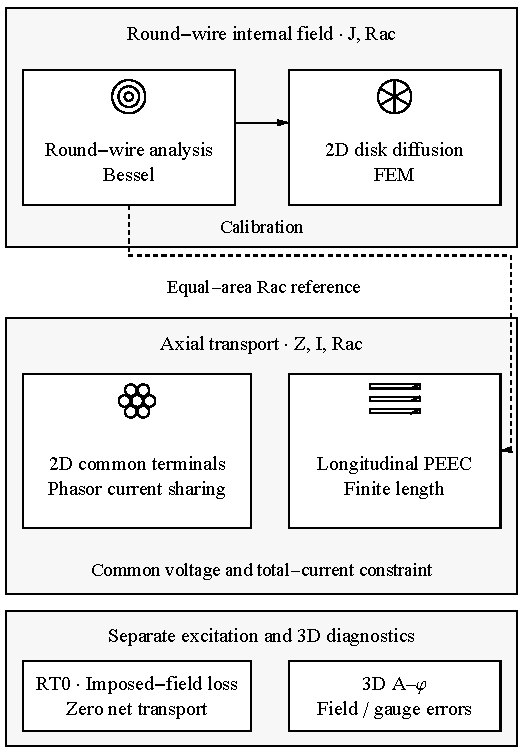
\includegraphics[width=\linewidth,height=.72\textheight,keepaspectratio]{../../assets/en/model_hierarchy.pdf}
\caption{Model hierarchy and comparable observables. Transport models are grouped by physical object and observable: round-wire internal fields support analytical and two-dimensional calibration, multistrand field–circuit models resolve common-terminal phasor currents, and longitudinal PEEC examines finite-length effects. Links identify internal-field calibration or equal-area resistance references. RT0 imposed-field loss and three-dimensional A–φ diagnostics occupy separate research scopes.}
\label{fig:model_hierarchy}
\end{figure}

% block-id: 01.automation.p1
\hypertarget{01.automation.p1}{}
Agent workflows connect source, Wolfram/Ansys MCP, bounded runners, and independent acceptance throughout the research. Six recorded case classes cover calibration, model construction and solution, cross-solver comparison, frequency extension, interface repair, and numerical failure diagnosis. This report connects the physical models to those execution records, showing how investigators can locate inputs, repeat calculations, and continue model development. \cite{CODEX,AGENTTOOLS,PYAEDTMCP}

\section{Physical Conventions and Model Hierarchy}
\label{chapter:02}

% block-id: 02.conventions.heading
\hypertarget{02.conventions.heading}{}
\subsection{Operating conditions and comparison quantities}

% block-id: 02.conventions.p1
\hypertarget{02.conventions.p1}{}
Calculations use SI units, the exp(jωt) time convention, and RMS phasors. Copper at 20 °C has conductivity σ=5.8×10⁷ S/m and relative permeability μr=1. The principal transport condition is 200 kHz and 20 A RMS, with zero independent imposed field. Strands are insulated along their lengths and connected in parallel at their ends. Resistance and loss are normalized by axial length; actual strand arc lengths enter copper volume and DC resistance separately. Finite-segment terminal voltage is measured in V, while the two-dimensional axial terminal field is measured in V/m, with the chosen axial length connecting the two.

% block-id: 02.conventions.p2
\hypertarget{02.conventions.p2}{}
The original Q1 round wire, 2 mm in diameter, provides an analytical calibration. Its copper area is 3.141593 mm² and its mean DC current density at 20 A is 6.366198 A/mm², exceeding the specified limit of 4 A/mm². Q2 therefore requires at least 5 mm² copper cross-section. For 640 strands of copper diameter 0.100 mm, the ideal circular area is 5.026548 mm². Each strand in the two-dimensional model is represented by a 64-sided polygon, giving an actual copper area of \metric{coax_area} mm². Equal-copper comparisons use this discrete area so that the electromagnetic reference incorporates the same geometric approximation.

% block-id: 02.conventions.p3
\hypertarget{02.conventions.p3}{}
For unequal strand arc lengths, parallel conductances determine DC resistance and the sum of strand area–length products determines copper volume, as in \eqref{eq:E01}. We examine absolute AC resistance, Rac/Rdc, copper loss, and complex current sharing. Equation \eqref{eq:E02} gives RMS Joule loss and defines resistance from copper dissipation under pure transport excitation. The supplementary RT0 case uses an independent imposed field and zero net transport, so its absorbed power is reported separately as imposed-field loss.

% block-id: 02.maxwell.heading
\hypertarget{02.maxwell.heading}{}
\subsection{Maxwell}

% block-id: 02.maxwell.p1
\hypertarget{02.maxwell.p1}{}
In the magnetoquasistatic approximation, conduction dominates displacement current and charge continuity gives \(\nabla\)·J=0. With exp(jωt), Faraday’s law is \(\nabla\)×E=−jωB and Ohm’s law is J=σE. Materials, excitation, return, and boundary conditions define a boundary-value problem. Mapping its comparable observables to the next discretization establishes the verification sequence used here.

% block-id: 02.hierarchy.heading
\hypertarget{02.hierarchy.heading}{}
\subsection{Model hierarchy and verification relationships}

% block-id: 02.hierarchy.p1
\hypertarget{02.hierarchy.p1}{}
The models are related as shown in Fig.~\ref{fig:model_hierarchy}. Analytical round-wire and two-dimensional diffusion models share the long, straight internal-field problem, allowing radial current and internal resistance to be compared. The two-dimensional common-terminal model additionally retains intrastand distributions, interstrand currents, and a controlled return, supporting field–circuit analysis of a specified cross-section. Longitudinal PEEC uses a finite-length partial-inductance kernel to examine the effect of length on axial currents. The three-component RT0 model uses imposed-field absorption in a cuboid to test three-dimensional continuity and discrete operators. Transposition paths and actual end regions require corresponding longitudinal or transverse degrees of freedom in subsequent structural research.

% block-id: 02.hierarchy.p2
\hypertarget{02.hierarchy.p2}{}
Verification comprises equation solution, physical constraints, power consistency, and parameter sensitivity. Targets are 10⁻⁸ for true linear residuals, common-terminal conditions, and total complex current; 0.1\% for independent power balance; and 1\% for changes in mesh, segmentation, boundary, and length. Analytical reference values and current/power integrals use thresholds of 10⁻⁶ and 10⁻⁸, respectively. The RT0 GMRES true-residual target is 10⁻¹¹, its quadrature-sensitivity target is 0.1\%, and same-model CPU/GPU matrix and complex-current comparisons use 10⁻¹⁰.

% block-id: 02.hierarchy.p3
\hypertarget{02.hierarchy.p3}{}
These checks answer different questions. Residuals measure the accuracy of the discrete-system solution, power balance tests field–circuit and postprocessing consistency, and parameter sensitivity describes changes over specified perturbations. Model omissions, boundary approximations, and experimental deviations require their own evidence. We therefore distinguish numerical checks from physical applicability and interpret finite sensitivity studies as local validation rather than a common upper bound on total model error.

% block-id: 02.equation.E01
\hypertarget{02.equation.E01}{}
\hypertarget{E01}{}
\begin{equation}
\begin{gathered}
R_{\mathrm{dc}}=\left(\sum_{k=1}^{N}\frac{\sigma A_k}{\ell_k}\right)^{-1} \\
V_{\mathrm{Cu}}=\sum_{k=1}^{N}A_k\ell_k
\end{gathered}
\tag{1}\label{eq:E01}
\end{equation}

% block-id: 02.equation.E02
\hypertarget{02.equation.E02}{}
\hypertarget{E02}{}
\begin{equation}
\begin{gathered}
P_{\mathrm{Cu}}=\int_{\Omega_{\mathrm{Cu}}}|\mathbf J|^2/\sigma\,\mathrm d\Omega \\
R_{\mathrm{ac}}=P_{\mathrm{Cu}}/|I_t|^2 \\
r_{\mathrm{ac}}=R_{\mathrm{ac}}/L_z
\end{gathered}
\tag{2}\label{eq:E02}
\end{equation}

\section{Round-Wire Analysis and Two-Dimensional Calibration}
\label{chapter:03}

% block-id: 03.round_derivation.heading
\hypertarget{03.round_derivation.heading}{}
\subsection{Round-wire radial equation and normalization}

% block-id: 03.round_derivation.p1
\hypertarget{03.round_derivation.p1}{}
Axial current inside a long straight round wire satisfies (1/r)d(r dJz/dr)/dr=κ²Jz. Finiteness at the axis selects I\(_0\)(κr), and the total complex-current constraint together with \(\int\)\(_0\)\(^a\)rI\(_0\)(κr)dr=aI\(_1\)(κa)/κ fixes its coefficient. Surface axial electric field divided by total current gives internal impedance per unit length. An independent Joule integral of current density checks the relationship between its real part and loss. The derivation uses the same RMS phasors as the main text.

% block-id: 03.analytic.heading
\hypertarget{03.analytic.heading}{}
\subsection{Round-wire internal-field calibration}

% block-id: 03.analytic.p1
\hypertarget{03.analytic.p1}{}
The radial current and internal impedance of a long straight round wire follow \eqref{eq:E03}. At 200 kHz, the skin depth δ=\metric{skin_depth} mm is approximately 0.148 times the radius, and current concentrates near the surface. DC resistance is \metric{q1_rdc} mΩ/m, AC resistance is \metric{q1_rac} mΩ/m, and Rac/Rdc=3.64720, giving a loss of \metric{q1_loss} W/m. The radial profiles and cross-sectional magnitude appear in Fig.~\ref{fig:q1_profile} and Fig.~\ref{fig:q1_cross_section}. Radial phase is continuously unwrapped, showing the amplitude attenuation and phase change associated with skin diffusion. The analytical impedance concerns the conductor's internal field.

% block-id: 03.analytic.p2
\hypertarget{03.analytic.p2}{}
Independent two-dimensional disk diffusion uses three meshes with 353, 1389, and 5573 nodes, normalized by total complex current. With refinement, relative Rac error against analysis decreases from 7.05×10⁻³ to 2.30×10⁻⁴ and finally 1.79×10⁻⁶. The finest-grid relative power-integral difference is 3.07×10⁻⁶, as shown in Fig.~\ref{fig:q1_fem_error}. These results verify discretization, normalization, and power postprocessing for the isolated round-wire internal-field problem. The cross-sectional illustration uses linear interpolation of analytical radial samples and an axisymmetric mapping; subsequent multistrand models use their actual conductor field solutions.

% block-id: 03.equation.E03
\hypertarget{03.equation.E03}{}
\hypertarget{E03}{}
\begin{equation}
\begin{gathered}
\delta=(\pi f\mu\sigma)^{-1/2} \\
\kappa=(1+j)/\delta \\
J_z(r)=\frac{I_t\kappa I_0(\kappa r)}{2\pi a I_1(\kappa a)} \\
z_{\mathrm{int}}=\frac{\kappa I_0(\kappa a)}{2\pi a\sigma I_1(\kappa a)}
\end{gathered}
\tag{3}\label{eq:E03}
\end{equation}

% block-id: 03.figure.q1_profile
\hypertarget{03.figure.q1_profile}{}
\begin{figure}[!htbp]
\centering
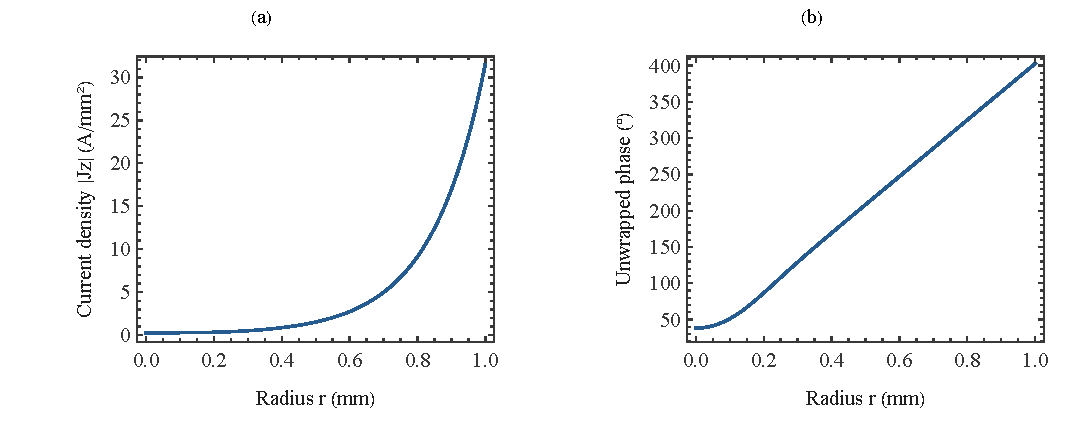
\includegraphics[width=\linewidth,height=.72\textheight,keepaspectratio]{../../assets/en/q1_profile.pdf}
\caption{Round-wire radial current magnitude and phase. The copper conductor has diameter 2 mm and carries 20 A RMS at 200 kHz. (a) RMS magnitude; (b) continuously displayed phase. Phase is displayed with a continuous radial lift, while magnitude retains RMS normalization. Radial samples come from preserved Bessel analytical data.}
\label{fig:q1_profile}
\end{figure}

% block-id: 03.figure.q1_cross_section
\hypertarget{03.figure.q1_cross_section}{}
\begin{figure}[!htbp]
\centering
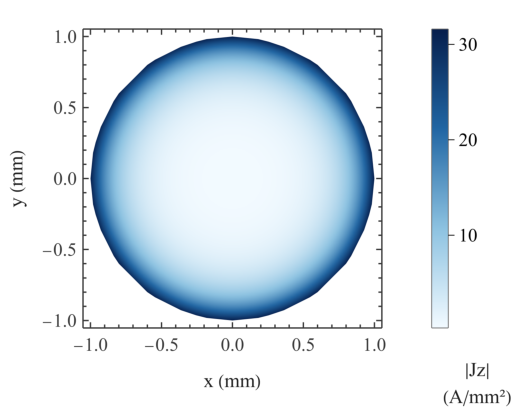
\includegraphics[width=\linewidth,height=.72\textheight,keepaspectratio]{../../assets/en/q1_cross_section.pdf}
\caption{Analytical round-wire cross-sectional magnitude. The copper conductor has diameter 2 mm and carries 20 A RMS at 200 kHz. The color scale represents axial RMS current density. Radial samples are linearly interpolated and mapped axisymmetrically. Coordinates are displayed in millimetres and current density in A/mm².}
\label{fig:q1_cross_section}
\end{figure}

% block-id: 03.figure.q1_fem_error
\hypertarget{03.figure.q1_fem_error}{}
\begin{figure}[!htbp]
\centering
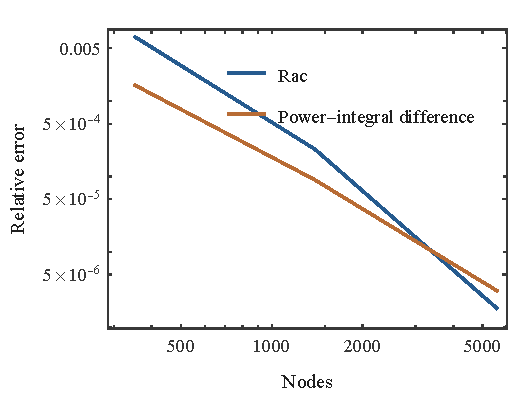
\includegraphics[width=\linewidth,height=.72\textheight,keepaspectratio]{../../assets/en/q1_fem_error.pdf}
\caption{Round-wire two-dimensional calibration errors. The copper conductor has diameter 2 mm and carries 20 A RMS at 200 kHz. Three grids and independent power integrals concern the same internal-field problem. Resistance is referenced to the internal Bessel solution of the same round wire. Power is evaluated by independent integration over the material region.}
\label{fig:q1_fem_error}
\end{figure}

\section{Multistrand Common-Terminal Circuits and Sharing Criterion}
\label{chapter:04}

% block-id: 04.common.heading
\hypertarget{04.common.heading}{}
\subsection{Common-terminal coupling and uniform complex currents}

% block-id: 04.common.p1
\hypertarget{04.common.p1}{}
The common endpoints, strand branches, and return are related in Fig.~\ref{fig:common_terminal}. Let Z be the coupled impedance matrix of a specified linear model, e the independently induced voltage, i the complex strand currents, and V the common terminal voltage. The port equation Zi+e=V1 and total-current constraint 1\(^{\mathrm T}\)i=It form \eqref{eq:E04}. Solving the augmented system yields both magnitude and phase; It/N serves as a reference for the resulting current distribution.

% block-id: 04.common.p2
\hypertarget{04.common.p2}{}
When the augmented system has a unique solution, substitution of i=(It/N)1 shows that uniform currents exist if and only if every component of (It/N)Z1+e is equal. Projecting this vector onto the subspace orthogonal to 1 gives \eqref{eq:E05}. Without an independent imposed field, the condition reduces to equal row sums of Z; with an imposed field, the induced term also determines current sharing. This necessary and sufficient condition applies to the selected impedance model and terminal conditions, expressing the effect of transposition through changes in coupling and induced voltages.

% block-id: 04.common.p3
\hypertarget{04.common.p3}{}
The two-dimensional common-terminal FEM solves the shared axial terminal field jointly with Az degrees of freedom. In conductors, Jz=σ(v−u), where both v and the saved variable u are expressed in V/m; the return conductor uses its corresponding terminal field. Current and loss are integrated on material-tagged linear triangles after coordinates are converted from mm to m. Strand currents, bundle loss, return loss, and copper area are independently compared with the original field–circuit results, treating air and conductor regions separately.

% block-id: 04.sharing_derivation.heading
\hypertarget{04.sharing_derivation.heading}{}
\subsection{Derivation of the uniform complex-current condition}

% block-id: 04.sharing_derivation.p1
\hypertarget{04.sharing_derivation.p1}{}
If a uniform-current solution exists, substituting i=(It/N)1 into the port equation makes all components of (It/N)Z1+e equal, establishing necessity of the projection condition. Conversely, when the projection condition holds, this vector equals a scalar V times 1. The uniform-current vector then satisfies both the port equation and the total-current constraint; uniqueness of the augmented solution makes it the actual solution, establishing sufficiency. Numerical results use sqrt(mean(|ik−It/N|²))/|It/N| for normalized RMS complex-current deviation and show individual magnitudes and phases.

% block-id: 04.coax_results.heading
\hypertarget{04.coax_results.heading}{}
\subsection{Common-terminal currents and loss in a 640-strand straight bundle}

% block-id: 04.coax_results.p1
\hypertarget{04.coax_results.p1}{}
Three meshes and variations of return distance and exterior domain complete 23 checks. The final mesh refinement changes Rac by 0.011902\%; return-distance and exterior-domain changes are 0.000495\% and 0.000270\%, respectively, as shown in Fig.~\ref{fig:coax640_mesh}. These changes remain below the 1\% comparison target over the tested perturbations, supporting numerical stability of the specified two-dimensional common-terminal result. Its applicability is a straight two-dimensional bundle with a controlled return; finite end regions and longitudinal coupling in actual wound structures require further verification.

% block-id: 04.coax_results.p2
\hypertarget{04.coax_results.p2}{}
Fig.~\ref{fig:coax640_currents} shows current magnitude and phase by physical strand identity, with It/N as the equal-current reference. Magnitude and phase jointly determine each strand's contribution to total transport current, so current sharing is evaluated using complex currents. Fig.~\ref{fig:coax640_fields} gives the corresponding cross-sectional fields, connecting strand statistics with spatial position. In this axially invariant straight bundle, the skin-effect scale within each fine strand coexists with collective current redistribution caused by magnetic coupling across the bundle. Longitudinal transposition requires a separate representation of position changes.

% block-id: 04.interpretation.heading
\hypertarget{04.interpretation.heading}{}
\subsection{Interpretation}

% block-id: 04.interpretation.p1
\hypertarget{04.interpretation.p1}{}
The 640-strand section distinguishes the skin-effect scale of an individual fine strand from collective current redistribution in the bundle. Inner and outer strands experience different magnetic coupling; under a common terminal field, this difference appears in current magnitude and phase. DC area supplies a reference for copper utilization, the bundle Joule integral gives transport loss, and the separate return integral describes energy allocation across the complete field–circuit system.

% block-id: 04.quantitative.p1
\hypertarget{04.quantitative.p1}{}
The actual copper cross-section of the two-dimensional 640-strand model is \metric{coax_area} mm². Bundle AC resistance is \metric{coax_rac} mΩ per axial metre, bundle loss is \metric{coax_bundle_loss} W per axial metre, and return loss is \metric{coax_return_loss} W per axial metre. Separate integration identifies dissipation in the bundle and return. The common axial terminal field is \metric{coax_voltage_re}+j(\metric{coax_voltage_im}) V/m. Complex strand currents sum to 20 A RMS, while their normalized RMS complex-current deviation is \metric{coax_spread}, demonstrating substantial interstrand differences in this common-terminal straight bundle.

% block-id: 04.equation.E04
\hypertarget{04.equation.E04}{}
\hypertarget{E04}{}\begin{equation}\begin{bmatrix} Z&-\mathbf1\\ \mathbf1^T&0\end{bmatrix}\begin{bmatrix}\mathbf i\\V\end{bmatrix}=\begin{bmatrix}-\mathbf e\\I_t\end{bmatrix}\tag{4}\label{eq:E04}\end{equation}

% block-id: 04.equation.E05
\hypertarget{04.equation.E05}{}
\hypertarget{E05}{}
\begin{equation}
\begin{gathered}
Q=I_N-\mathbf1\mathbf1^T/N \\
Q\left[(I_t/N)Z\mathbf1+\mathbf e\right]=\mathbf0
\end{gathered}
\tag{5}\label{eq:E05}
\end{equation}

% block-id: 04.figure.common_terminal
\hypertarget{04.figure.common_terminal}{}
\begin{figure}[!htbp]
\centering
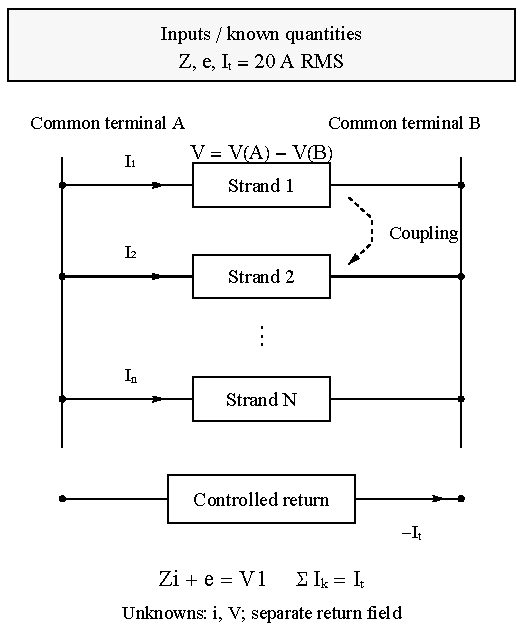
\includegraphics[width=\linewidth,height=.72\textheight,keepaspectratio]{../../assets/en/common_terminal.pdf}
\caption{Multistrand common terminals and return. Strands are insulated along their paths and connected in parallel at both ends; their phasor currents follow from the common voltage and total-current constraints. The coupling matrix Z and excitation term e contain the impedance and field contributions retained by the model. The controlled return carries the opposite total current and has its own terminal field. Known inputs and unknown currents and voltage are identified.}
\label{fig:common_terminal}
\end{figure}

% block-id: 04.figure.coax640_currents
\hypertarget{04.figure.coax640_currents}{}
\begin{figure}[!htbp]
\centering
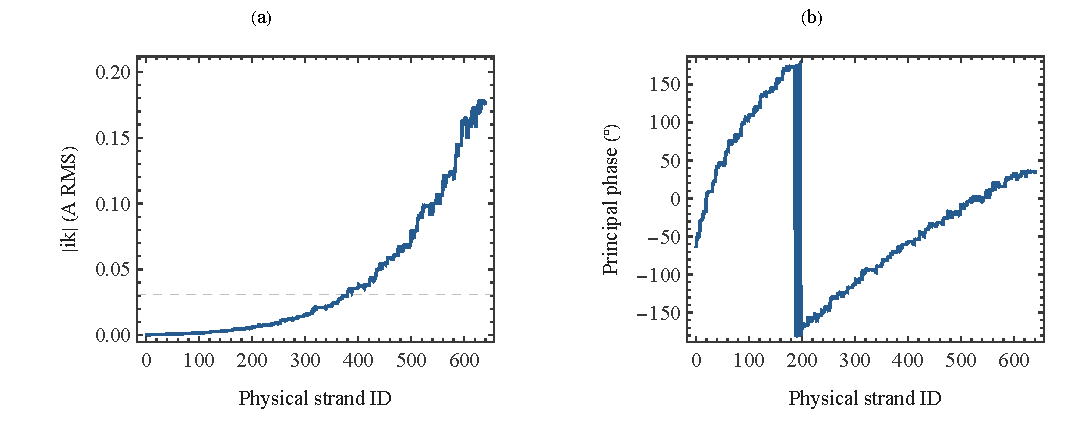
\includegraphics[width=\linewidth,height=.72\textheight,keepaspectratio]{../../assets/en/coax640_currents.pdf}
\caption{640-strand common-terminal complex current sharing. (a) Magnitude; (b) phase, ordered by physical strand identity. A dashed line marks the comparison reference It/N. Magnitude and phase use identical physical strand numbering.}
\label{fig:coax640_currents}
\end{figure}

% block-id: 04.figure.coax640_fields
\hypertarget{04.figure.coax640_fields}{}
\begin{figure}[!htbp]
\centering
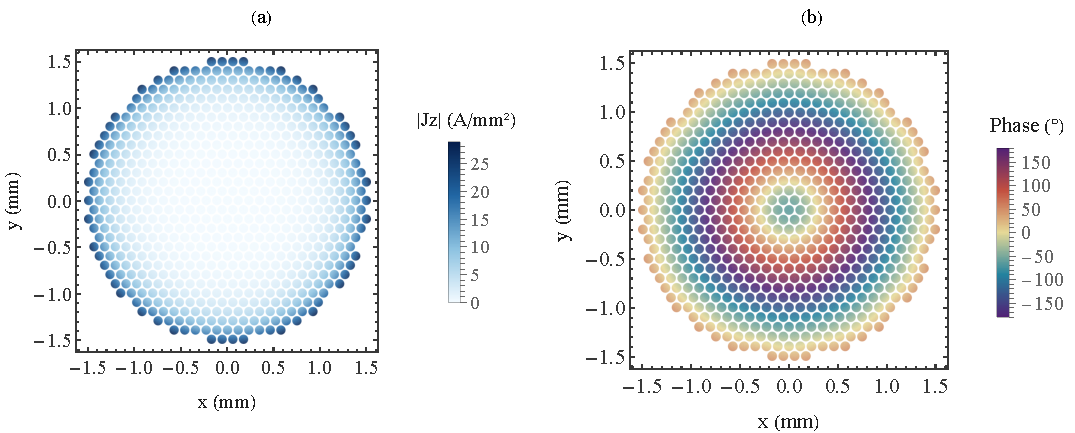
\includegraphics[width=\linewidth,height=.72\textheight,keepaspectratio]{../../assets/en/coax640_fields.pdf}
\caption{640-strand two-dimensional cross-sectional current density. (a) RMS magnitude; (b) phase, with material markers identifying strands. Current is reconstructed as Jz=σ(v−u) from original nodal and terminal fields. Independent power uses linear-triangle mass integration, while visualization samples cell centers.}
\label{fig:coax640_fields}
\end{figure}

% block-id: 04.figure.coax640_mesh
\hypertarget{04.figure.coax640_mesh}{}
\begin{figure}[!htbp]
\centering
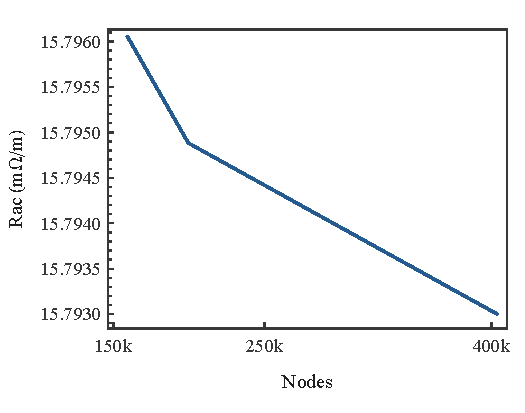
\includegraphics[width=\linewidth,height=.72\textheight,keepaspectratio]{../../assets/en/coax640_mesh.pdf}
\caption{640-strand mesh and boundary sensitivities. Mesh, return, and exterior tests each vary one factor. Variation is normalized from resistance differences between the specified adjacent cases. Mesh, return distance, and exterior size use separate sequences.}
\label{fig:coax640_mesh}
\end{figure}

\section{Transposition Models, Real Geometry, and Equal-Copper Comparisons}
\label{chapter:05}

% block-id: 05.geometry.heading
\hypertarget{05.geometry.heading}{}
\subsection{Geometry sampling and discrete transposition}

% block-id: 05.geometry.p1
\hypertarget{05.geometry.p1}{}
Fig.~\ref{fig:geometry_comparison} shows straight, single-level, traditional multilevel and cross-layer centerlines. The geometry records preserve strand identity, periodicity, clearance, curvature, actual arc length and copper volume. Axial sampling at 400, 800 and 1600 points and 60 checks support sampling consistency for these quantities. The illustrated 24-strand structure with a copper diameter of 0.100 mm has a nominal copper area of approximately 0.1885 mm² and demonstrates geometry construction. A structure meeting the minimum 5 mm² copper area requires separate construction and verification. Three-dimensional views reveal spatial paths; the corresponding field-circuit model evaluates electromagnetic performance.

% block-id: 05.geometry.p2
\hypertarget{05.geometry.p2}{}
The current DTM/iDTM demonstration uses the additive discrete blocks in \eqref{eq:E06}. For the same weighted impedance blocks, their sum is invariant to ordering; this implementation therefore checks identity mappings and circuit accumulation of the specified blocks. Comparing actual transposition paths additionally requires longitudinal position changes, noncommuting relationships between levels, local fields, and terminal conditions. These assumptions determine comparability with the literature \cite{P01,N01}.

% block-id: 05.dtm_derivation.heading
\hypertarget{05.dtm_derivation.heading}{}
\subsection{Mapping strand identity to cross-sectional position}

% block-id: 05.dtm_derivation.p1
\hypertarget{05.dtm_derivation.p1}{}
Let Ps map fixed physical strand identities to spatial positions in cross-section s. Local currents are Ps i, and local voltages transformed back to identity coordinates are Ps\(^{\mathrm T}\)ZsPs i. Summing in series with segment lengths Δzs gives \eqref{eq:E06}. Position and identity are retained separately; K, 2K, and 4K segmentation comparisons use the same trajectory and strands. Periodicity, clearance, and curvature check the paths, while actual arc lengths and copper volume quantify material use.

% block-id: 05.report_geometry.heading
\hypertarget{05.report_geometry.heading}{}
\subsection{Geometry Sampling and Equal-Copper Checks}

% block-id: 05.report_geometry.p1
\hypertarget{05.report_geometry.p1}{}
Trajectory recovery preserves physical strand IDs instead of renaming strands by cross-sectional order. Period checks distinguish position closure from identity permutation; gap and curvature checks use physical units, and arc length is integrated from sampled paths and compared with doubled sampling. Copper volume and DC resistance use actual strand lengths; the axial length is not substituted for every helical branch. Local cropping and display subsampling are recorded under the publication run, while complete original centerlines remain available.

% block-id: 05.report_geometry.p2
\hypertarget{05.report_geometry.p2}{}
Equal-copper comparisons identify circular nominal area, discretized actual area, and the outer envelope occupied by insulation. At the same nominal area, longer arc length increases copper volume per axial metre and the resistive path length. Geometric complexity itself supplies no evidence of electromagnetic improvement. The 640-strand candidate trajectories and 7/24-strand construction demonstrations serve different scales, and public materials should retain that distinction.

% block-id: 05.equation.E06
\hypertarget{05.equation.E06}{}
\hypertarget{E06}{}\begin{equation}Z_{\mathrm{tot}}=\sum_{s=1}^{K}\Delta z_s P_s^T Z_s P_s\tag{6}\label{eq:E06}\end{equation}

% block-id: 05.figure.geometry_comparison
\hypertarget{05.figure.geometry_comparison}{}
\begin{figure}[!htbp]
\centering
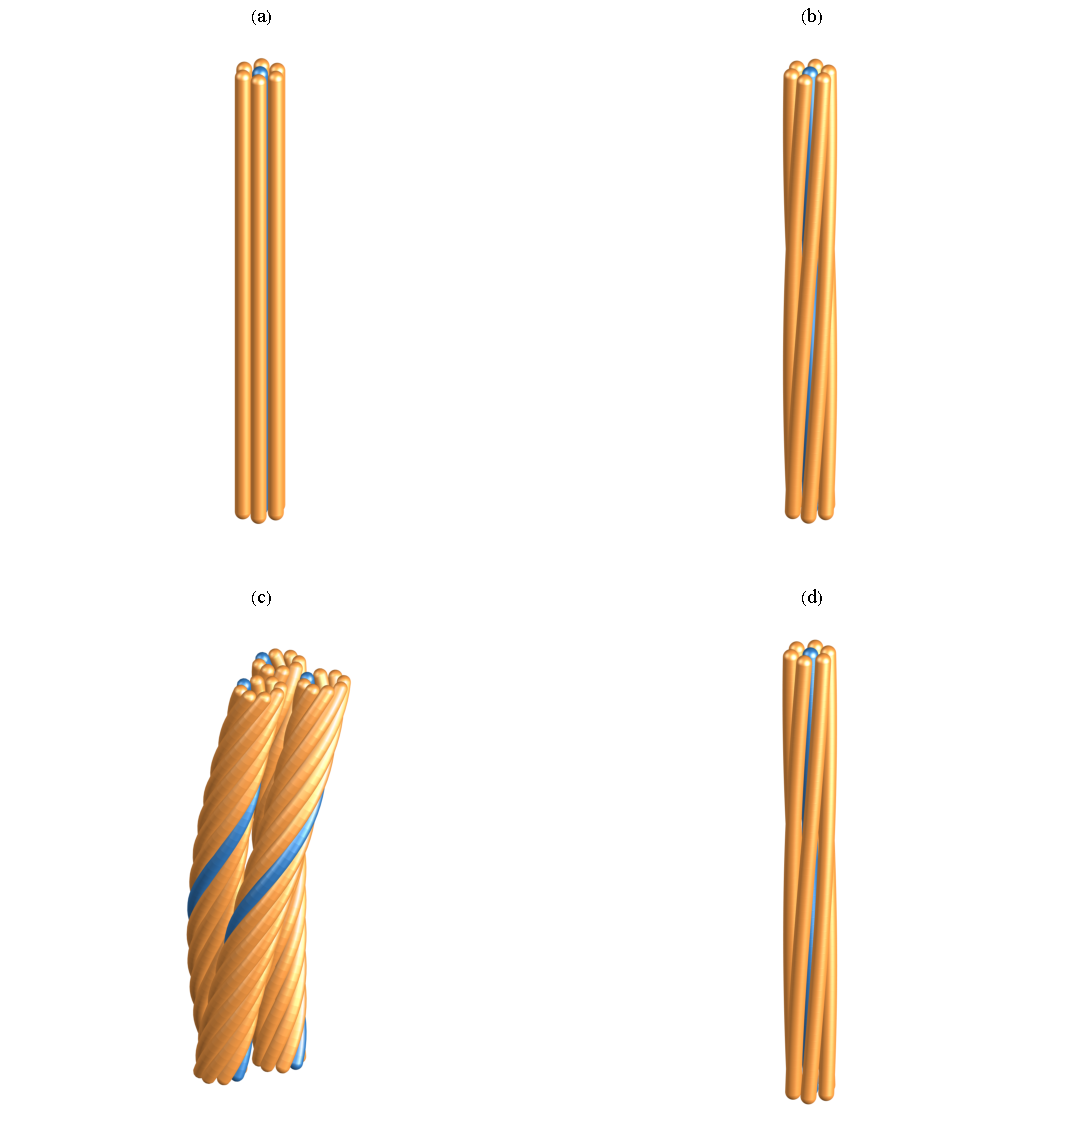
\includegraphics[width=\linewidth,height=.72\textheight,keepaspectratio]{../../assets/en/geometry_comparison.pdf}
\caption{Three-dimensional strand centerline structures. Panels show straight, single-level, local multilevel, and cross-layer structures. The 24-strand structures use a copper diameter of 0.100 mm, and the multilevel panel shows a 3 mm detail. Blue markers preserve selected physical strand identities.}
\label{fig:geometry_comparison}
\end{figure}

\section{Finite-Length Longitudinal PEEC}
\label{chapter:06}

% block-id: 06.peec_method.heading
\hypertarget{06.peec_method.heading}{}
\subsection{Finite-length longitudinal PEEC}

% block-id: 06.peec_method.p1
\hypertarget{06.peec_method.p1}{}
Longitudinal PEEC divides the cross-section into volume filaments, each carrying an axial complex current density uniform along its length. Ohmic resistance and finite-volume partial inductance follow \eqref{eq:E08}, forming Z=R+jωL before the common-port and total-current constraints in \eqref{eq:E04} are applied. The counts 1264 and 5024 denote volume-filament degrees of freedom in a continuous conductor. Differences between their currents represent internal current concentration within the longitudinal basis.

% block-id: 06.peec_method.p2
\hypertarget{06.peec_method.p2}{}
The longitudinal case has a nominal round-wire diameter of 2 mm. The m40 and m80 square filaments are 0.050 and 0.025 mm wide, giving actual cross-sectional areas of 3.16 and 3.14 mm². Sensitivity studies vary length, mutual integration, or self integration independently. The 1264-degree-of-freedom model uses one cross-section at lengths 0.16, 0.32, and 0.64 m. At fixed length, mutual quadrature order q is increased through 4, 6, and 8, while self-integration settings increase from 10/8 to 12/10. These pairs are AccuracyGoal and PrecisionGoal, the target absolute and relative precision digits. The 5024-degree-of-freedom model checks lengths 0.32 and 0.64 m and the same integration changes. Because the two cross-sectional discretizations have slightly different copper areas, each resistance is compared with its own equal-area Bessel reference; changes between discretizations include both discretization and area approximation.

% block-id: 06.peec_method.p3
\hypertarget{06.peec_method.p3}{}
The partial-inductance kernel includes magnetic coupling around finite conductors, whereas the Bessel solution gives the internal impedance of a long straight round wire. We compare their dissipative component Rac while retaining length and area conditions. The length study measures sensitivity of the current kernel and longitudinal basis. Transverse loops, curved strands, and actual end-current redistribution require extended degrees of freedom. The connection to FEM–PEEC coupling \cite{P03} lies in a joint field–circuit description; excitation, return, and field-feedback choices must be compared for each implementation.

% block-id: 06.peec_derivation.heading
\hypertarget{06.peec_derivation.heading}{}
\subsection{Longitudinal filament basis and kernel integration}

% block-id: 06.peec_derivation.p1
\hypertarget{06.peec_derivation.p1}{}
Within volume filament α, current density is constant at iα/Aα and directed axially. Volume integration of vector potential gives the induced electric field in a testing filament; integration along its length yields a symmetric partial-inductance matrix. Coincident points produce an integrable self-term singularity treated with dedicated precision settings, while mutual terms use a separate quadrature order. Ohmic resistance and jωL form the coupled matrix, solved jointly with common terminal voltage and total current. The basis determines the current directions represented by this model.

% block-id: 06.peec_results.heading
\hypertarget{06.peec_results.heading}{}
\subsection{Length and integration sensitivity of longitudinal PEEC}

% block-id: 06.peec_results.p1
\hypertarget{06.peec_results.p1}{}
For the 1264-degree-of-freedom model, resistances at 0.16, 0.32, and 0.64 m are 19.8992, 19.9586, and 19.9885 mΩ per axial metre. Consecutive length changes are 0.298640\% and 0.149482\%. The 5024-degree-of-freedom model changes by 0.148730\% from 0.32 to 0.64 m, as shown in Fig.~\ref{fig:peec_length}. Resistance changes decrease with increasing length, and all tested increments are below 1\%. The sequence characterizes sensitivity over the 0.16–0.64 m interval.

% block-id: 06.peec_results.p2
\hypertarget{06.peec_results.p2}{}
At 5024 degrees of freedom, Lz=0.64 m, mutual order q=4, and self-integration settings 12/10, Rac=\metric{peec_rac} mΩ per axial metre, Rac/Rdc=3.64472, and loss is 8.00510 W per axial metre. Resistance differs by 0.044582\% from the equal-area Bessel reference for this discretization. Fig.~\ref{fig:peec_cross_section} reconstructs the cross-sectional current distribution from saved filament currents and square cells, showing surface concentration within the conductor. These degrees of freedom discretize a continuous conductor; their current variation has a different meaning from current sharing among insulated strands.

% block-id: 06.peec_results.p3
\hypertarget{06.peec_results.p3}{}
Results for mutual order q=4\(\to\)6\(\to\)8 and self settings 10/8\(\to\)12/10 appear in Fig.~\ref{fig:peec_sensitivity}. Across both model sizes, the largest relative resistance change from mutual integration is 1.21×10⁻⁵ and the largest relative complex-current change is 1.60×10⁻⁵. Corresponding maxima for self integration are 6.75×10⁻¹¹ and 7.10×10⁻¹¹. Coarse-to-fine cross-sectional resistance changes at 0.32 and 0.64 m are 0.122127\% and 0.121376\%, respectively, and include changes in actual area. Thus integration settings have a smaller effect than length and cross-sectional discretization in these tests. Analytical references and sensitivities jointly support resistance calculation within the longitudinal model; actual end regions and transverse-current errors remain model-level research questions.

% block-id: 06.equation.E08
\hypertarget{06.equation.E08}{}
\hypertarget{E08}{}
\begin{equation}
\begin{gathered}
R_{\alpha\beta}=\delta_{\alpha\beta}\frac{L_z}{\sigma A_\alpha} \\
L_{\alpha\beta}=\frac{\mu}{4\pi A_\alpha A_\beta}\int_{V_\alpha}\int_{V_\beta}\frac{\hat{\mathbf t}_\alpha\cdot\hat{\mathbf t}_\beta}{|\mathbf r-\mathbf r'|}\,\mathrm dV\,\mathrm dV'
\end{gathered}
\tag{7}\label{eq:E08}
\end{equation}

% block-id: 06.figure.peec_cross_section
\hypertarget{06.figure.peec_cross_section}{}
\begin{figure}[!htbp]
\centering
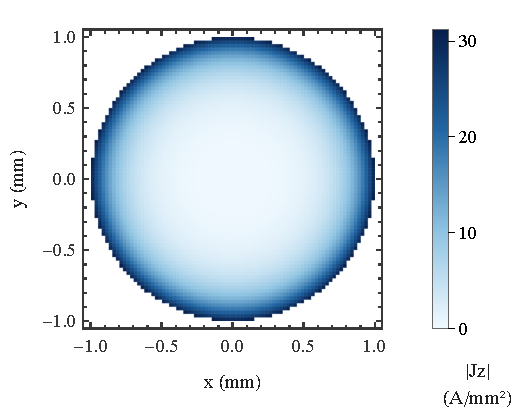
\includegraphics[width=\linewidth,height=.72\textheight,keepaspectratio]{../../assets/en/peec_cross_section.pdf}
\caption{Longitudinal PEEC cross-sectional current. Complex currents in square volume filaments reconstruct the RMS magnitude. The representative model contains 5024 longitudinal volume filaments and has axial length 0.64 m. Coordinates and material areas follow that level’s actual square-cell discretization.}
\label{fig:peec_cross_section}
\end{figure}

% block-id: 06.figure.peec_length
\hypertarget{06.figure.peec_length}{}
\begin{figure}[!htbp]
\centering
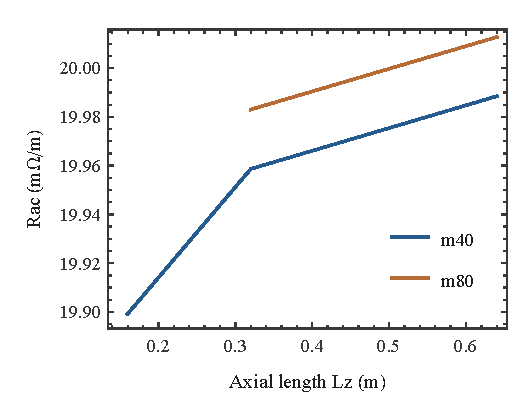
\includegraphics[width=\linewidth,height=.72\textheight,keepaspectratio]{../../assets/en/peec_length.pdf}
\caption{Longitudinal PEEC length sensitivity. Resistance per axial length is compared at archived lengths for the same cross-section. The 1264-degree-of-freedom model uses 0.16, 0.32, and 0.64 m, while 5024 degrees of freedom recheck the final two levels. Integration settings remain fixed within each length sequence.}
\label{fig:peec_length}
\end{figure}

% block-id: 06.figure.peec_sensitivity
\hypertarget{06.figure.peec_sensitivity}{}
\begin{figure}[!htbp]
\centering
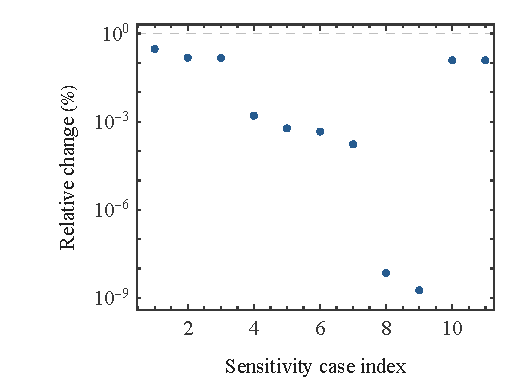
\includegraphics[width=\linewidth,height=.72\textheight,keepaspectratio]{../../assets/en/peec_sensitivity.pdf}
\caption{Longitudinal PEEC integration sensitivity. Mutual order and self accuracy are compared in separate single-factor tests. Mutual settings are q4, q6, and q8; self settings are 10/8 and 12/10. Comparisons retain the same cross-section and axial length.}
\label{fig:peec_sensitivity}
\end{figure}

\section{RT0 Three-Dimensional Imposed-Field Example}
\label{chapter:07}

% block-id: 07.rt0.p1
\hypertarget{07.rt0.p1}{}
The case is a homogeneous copper cuboid of 1×1×2 mm at 200 kHz, with imposed Bz=1 mT RMS and zero net transport. Three-component current is represented by face-flux degrees of freedom, with separate continuity, port-constraint, and imposed-field power checks. At quadrature q=14, meshes of 8192, 16000, and 27648 cells give losses of 0.927463, 0.933539, and 0.936927 mW. Consecutive refinement changes are 0.655090\% and 0.362916\%, below the 1\% target. Increasing the finest case to q=18 changes loss and complex face flux relatively by 1.55×10⁻⁸ and 1.39×10⁻⁸, respectively, below the 0.1\% quadrature target; see Fig.~\ref{fig:rt0_spatial}.

% block-id: 07.rt0.p2
\hypertarget{07.rt0.p2}{}
Sections and vectors in Fig.~\ref{fig:rt0_sections} and Fig.~\ref{fig:rt0_vectors} are reconstructed from saved face fluxes. Cell-center current is obtained by averaging opposite-face fluxes and dividing by face area. Cell-average loss density uses the full local RT0 overlap integral and therefore includes within-cell variation. Arrows show the real current at zero phase with one common length scale; color represents the complex RMS norm. Section locations and vector samples follow the figure annotations, while volume integration uses all cells.

% block-id: 07.rt0.p3
\hypertarget{07.rt0.p3}{}
Each mesh records 35 GMRES iterations and meets the 10⁻¹¹ true-residual target. Spatial and quadrature comparisons jointly support the fixed-cuboid imposed-field result. Applicability has yet to extend to curved Litz masks, independently validated boundary fluxes, and actual transport terminals. The original q=18 summary's missing metrics and failure status, CSV-based postprocessing acceptance, and resource records for dense and matrix-free implementations are retained separately to preserve the relationship between solution and interpretation.

% block-id: 07.figure.rt0_sections
\hypertarget{07.figure.rt0_sections}{}
\begin{figure}[!htbp]
\centering
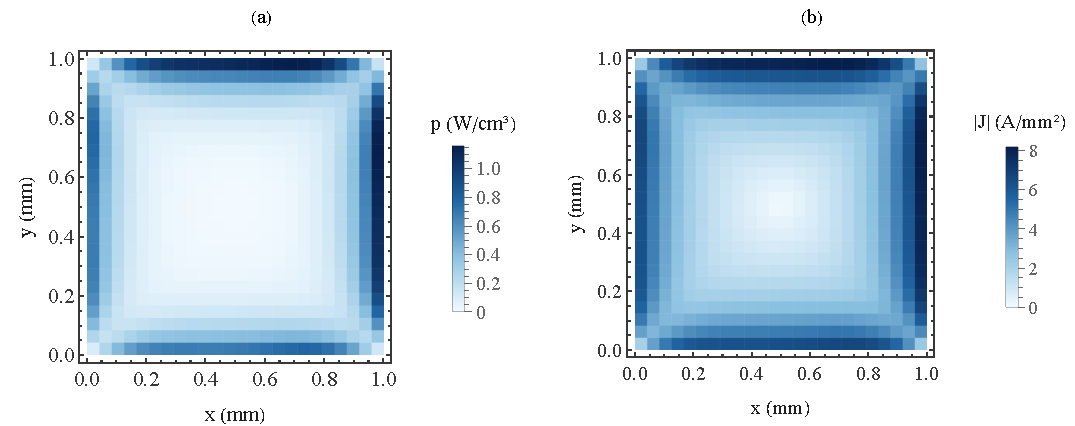
\includegraphics[width=\linewidth,height=.72\textheight,keepaspectratio]{../../assets/en/rt0_sections.pdf}
\caption{RT0 imposed-field current and loss sections. The 1×1×2 mm copper cuboid is excited at 200 kHz by a 1 mT RMS field with zero net transport. (a) Cell-average loss density; (b) complex RMS current norm. Current is reconstructed from opposing face fluxes, and cell-average loss uses RT0 overlap integration. Section positions and color scales follow the archived reconstruction definitions.}
\label{fig:rt0_sections}
\end{figure}

% block-id: 07.figure.rt0_vectors
\hypertarget{07.figure.rt0_vectors}{}
\begin{figure}[!htbp]
\centering
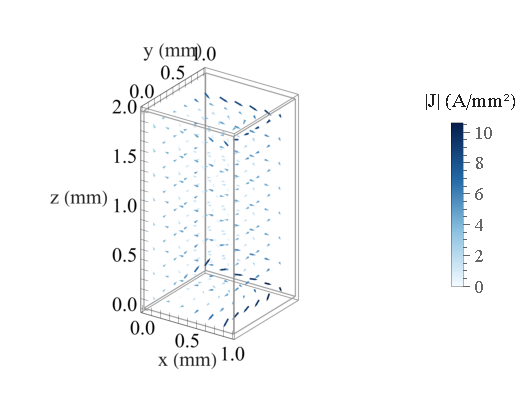
\includegraphics[width=\linewidth,height=.72\textheight,keepaspectratio]{../../assets/en/rt0_vectors.pdf}
\caption{RT0 reconstructed three-dimensional current vectors. The 1×1×2 mm copper cuboid is excited at 200 kHz by a 1 mT RMS field with zero net transport. Arrows show the real part at a fixed phase; color represents the complex RMS norm. Vectors use a common scale and sparse cell sampling. Cell and face-flux identities correspond in the preserved reconstruction data.}
\label{fig:rt0_vectors}
\end{figure}

% block-id: 07.figure.rt0_spatial
\hypertarget{07.figure.rt0_spatial}{}
\begin{figure}[!htbp]
\centering
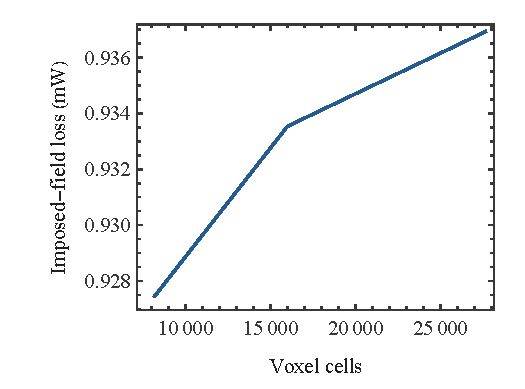
\includegraphics[width=\linewidth,height=.72\textheight,keepaspectratio]{../../assets/en/rt0_spatial.pdf}
\caption{RT0 spatial and integration comparisons. The 1×1×2 mm copper cuboid is excited at 200 kHz by a 1 mT RMS field with zero net transport. The q14 spatial sequence and final q18 comparison use the same imposed-field condition. The spatial sequence contains 8192, 16000, and 27648 cells. Integration is compared on the final successful grid.}
\label{fig:rt0_spatial}
\end{figure}

\section{Three-Dimensional A–φ Fields and Diagnostics}
\label{chapter:08}

% block-id: 08.aphi.p1
\hypertarget{08.aphi.p1}{}
The A–φ model recovers current using \eqref{eq:E07} from saved A and actual gradients of φ. The three cylinder meshes contain 1683, 3672, and 9108 nodes; results appear in Fig.~\ref{fig:aphi_gates}. Radial J calibration meets its target on the finest mesh, while φ and gauge residuals fail on all three; the two coarser meshes also fail the J target. Manufactured-solution checks support correspondence between the tested equations and implementation, while physical cylinder calibration reveals field–potential consistency questions requiring further research.

% block-id: 08.aphi.p2
\hypertarget{08.aphi.p2}{}
Fig.~\ref{fig:aphi_preserved} uses 128 explicitly identified nodal samples to display A, φ, J and the actual φ gradient at those locations. The reproduction materials retain boundary, scaling, derivative and postprocessing diagnostics, together with failure causes for direct factorization, out-of-core and iterative routes. These records help distinguish implementation problems from discretization errors. The current cylinder results have not passed physical acceptance.

% block-id: 08.equation.E07
\hypertarget{08.equation.E07}{}
\hypertarget{E07}{}\begin{equation}\mathbf J=-\sigma\left(j\omega\mathbf A+\nabla\phi\right)\tag{8}\label{eq:E07}\end{equation}

% block-id: 08.figure.aphi_preserved
\hypertarget{08.figure.aphi_preserved}{}
\begin{figure}[!htbp]
\centering
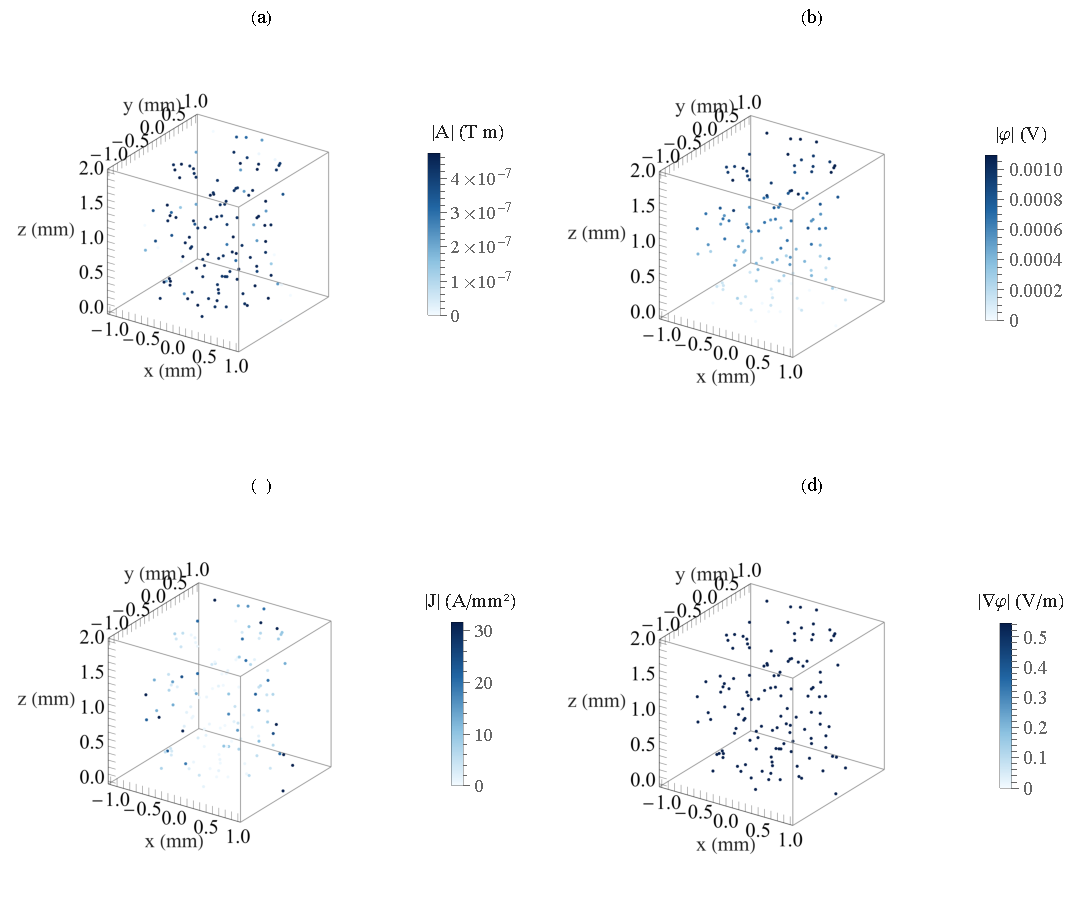
\includegraphics[width=\linewidth,height=.72\textheight,keepaspectratio]{../../assets/en/aphi_preserved.pdf}
\caption{Preserved A–φ field samples. Panels show A, φ, J, and the actual gradient of φ. The 128 selected nodes retain their sample identities. Color scales use magnitudes of the actual saved complex fields and derivatives.}
\label{fig:aphi_preserved}
\end{figure}

% block-id: 08.figure.aphi_gates
\hypertarget{08.figure.aphi_gates}{}
\begin{figure}[!htbp]
\centering
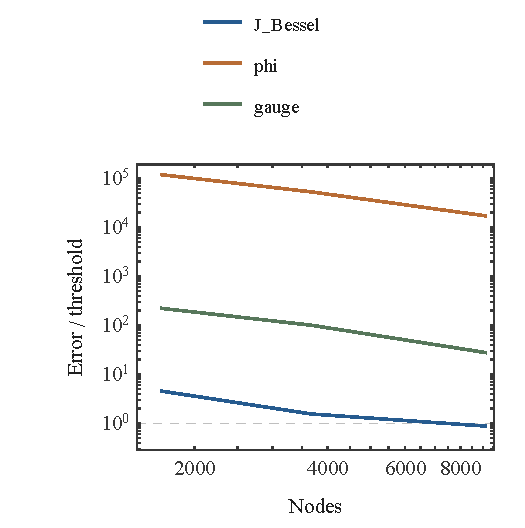
\includegraphics[width=\linewidth,height=.72\textheight,keepaspectratio]{../../assets/en/aphi_gates.pdf}
\caption{A–φ cylinder calibration metrics. Three grids and their metric targets are shown separately. The three cylinder levels contain 1683, 3672, and 9108 nodes. Errors are normalized by their respective acceptance targets, with the horizontal line indicating a unit ratio.}
\label{fig:aphi_gates}
\end{figure}

\section{Ansys Cases and Interface Verification}
\label{chapter:09}

% block-id: 09.ansys.p1
\hypertarget{09.ansys.p1}{}
The historical two-dimensional seven-strand port test uses 704 elements, two voltage basis solutions, and a third actual ±20 A field solution. Common terminal voltage, complex strand currents, and independent power establish field–circuit consistency on that mesh; current results appear in Fig.~\ref{fig:ansys_seven_current}. Validation concerns one mesh. Subsequent fixed-mesh and precision attempts have not completed the required three-level checks, and the native three-dimensional J-expression probe has not produced an acceptable physical solution.

% block-id: 09.ansys.p2
\hypertarget{09.ansys.p2}{}
Fig.~\ref{fig:ansys_limits} summarizes the verified Ansys Student v252 limits: up to 2000 triangles in two dimensions, 64000 volume elements and 8000 surface elements in three dimensions, and at most four processor cores. Interface capability, licensed model size and numerical accuracy separately constrain executable validation. Actual terminations, curved STL geometry and large bundles with sufficient copper area require licensing and mesh capacity appropriate to the target geometry, followed by sensitivity and power-balance checks.

% block-id: 09.figure.ansys_seven_current
\hypertarget{09.figure.ansys_seven_current}{}
\begin{figure}[!htbp]
\centering
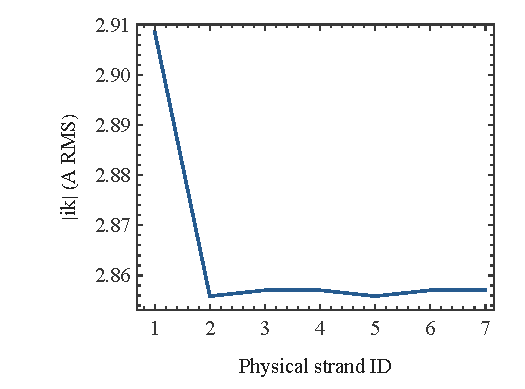
\includegraphics[width=\linewidth,height=.72\textheight,keepaspectratio]{../../assets/en/ansys_seven_current.pdf}
\caption{Ansys seven-strand two-dimensional complex currents. The valid 704-cell port short test provides strand magnitudes and phases. Currents use port records from the actual ±20 A field solution. Magnitudes and phases correspond to the same seven strand identities.}
\label{fig:ansys_seven_current}
\end{figure}

% block-id: 09.figure.ansys_limits
\hypertarget{09.figure.ansys_limits}{}
\begin{figure}[!htbp]
\centering
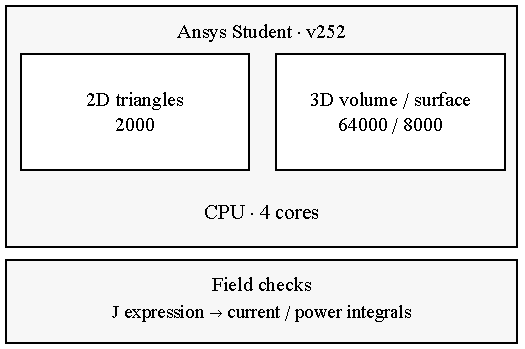
\includegraphics[width=\linewidth,height=.72\textheight,keepaspectratio]{../../assets/en/ansys_limits.pdf}
\caption{Ansys Student capacity and interface diagnostics. License capacity and field-check entry points for Ansys Student v252: 2000 triangles in two dimensions, 64000 volume and 8000 surface elements in three dimensions, and up to four compute cores. Capacity information is retained from rc.1 records; figure sources were checked on 2026-10-15.}
\label{fig:ansys_limits}
\end{figure}

% block-id: 09.ansys.rc2
\hypertarget{09.ansys.rc2}{}
The rc.2 records additionally complete two-dimensional Maxwell construction, solution, and project readback through PyAEDT-MCP, with task cancellation and linked restart records. A seven-strand straight-bundle comparison with Wolfram aligns cross-section, material, frequency, return, and total-current constraints. Relative complex-current L2 and bundle Rac differences are 0.0106814\% and 0.00132823\%, respectively. The implementations use independent meshes, Maxwell performs one adaptive pass, and spatial and boundary convergence remain to be checked. This success establishes the corresponding two-dimensional port workflow; three-dimensional interfaces and transposed structures with sufficient copper require their own field solutions and acceptance. \cite{PYAEDTMCP,PYAEDT}

\section{Implementation, CPU/GPU Comparison, and Resources}
\label{chapter:10}

% block-id: 10.compute.heading
\hypertarget{10.compute.heading}{}
\subsection{CPU/GPU numerical comparison and computational scale}

% block-id: 10.compute.p1
\hypertarget{10.compute.p1}{}
With identical model, discretization, and integration settings, the 5024-degree-of-freedom CPU/GPU partial-inductance matrices differ relatively by 7.48×10⁻¹⁶ and their complex currents by 7.78×10⁻¹⁴. The 1264-degree-of-freedom case also meets the 10⁻¹⁰ comparison threshold, as shown in Fig.~\ref{fig:gpu_equivalence}. These results establish numerical agreement between the two implemented algorithms for the compared matrices and port solutions. Performance comparisons additionally require matching timing boundaries; stage times and resource samples are retained, while physical conclusions rely on the model checks described above.

% block-id: 10.compute.p2
\hypertarget{10.compute.p2}{}
Fig.~\ref{fig:resource_memory} shows sampled memory usage for identifiable owned process trees; short peaks between samples may exceed the displayed curve. At larger scales, the 9856-degree-of-freedom case retains recoverable partial currents and related results, while its complete matrix, common voltage and full-field coverage are itemized in the data inventory. Cases with 20108 or more degrees of freedom record resource requirements and termination boundaries. These records inform the cost of further computation; complete numerical verification rests on cases with the corresponding acceptance data.

% block-id: 10.workflow.heading
\hypertarget{10.workflow.heading}{}
\subsection{Computation and document construction}

% block-id: 10.workflow.p1
\hypertarget{10.workflow.p1}{}
Research entry points read model inputs and solver settings and produce run records and corresponding checks. Publication entry points read saved quantities, figures and canonical LaTeX prose to generate Markdown reading editions and compile preview PDFs. Input, source, and output hashes identify each build. Individual figures retain vector curves and font information, while composites record panel identities and layout parameters. The following source table links observables in the text to specific files and acceptance records.

% block-id: 10.figure.gpu_equivalence
\hypertarget{10.figure.gpu_equivalence}{}
\begin{figure}[!htbp]
\centering
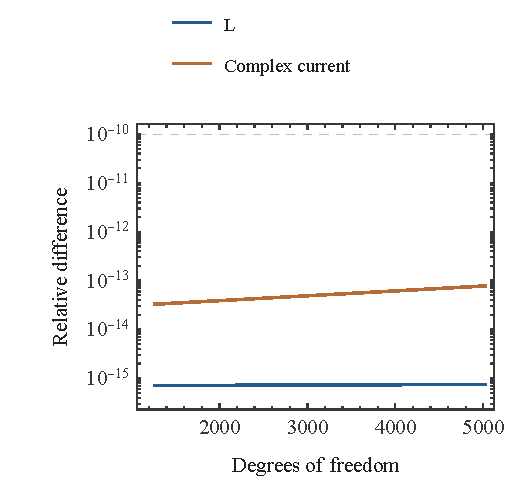
\includegraphics[width=\linewidth,height=.72\textheight,keepaspectratio]{../../assets/en/gpu_equivalence.pdf}
\caption{CPU/GPU same-model numerical comparison. Relative matrix and complex-current differences use identical discretization and integration. Relative differences are computed separately for 1264 and 5024 degrees of freedom. The horizontal reference is the 10⁻¹⁰ algorithm-comparison target.}
\label{fig:gpu_equivalence}
\end{figure}

% block-id: 10.figure.resource_memory
\hypertarget{10.figure.resource_memory}{}
\begin{figure}[!htbp]
\centering
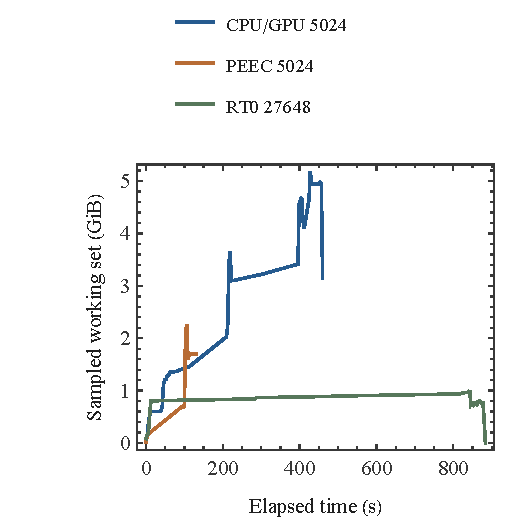
\includegraphics[width=\linewidth,height=.72\textheight,keepaspectratio]{../../assets/en/resource_memory.pdf}
\caption{Attributable process-tree resource curves. Curves use archived time and memory samples. Time is measured from the start of each corresponding run. Memory is the sampled working set of the attributable process tree.}
\label{fig:resource_memory}
\end{figure}

\section{General Discussion}
\label{chapter:11}

% block-id: 11.discussion.heading
\hypertarget{11.discussion.heading}{}
\subsection{Interpretation of current sharing and loss}

% block-id: 11.discussion.p1
\hypertarget{11.discussion.p1}{}
The three result levels answer the questions posed in the introduction. Round-wire analysis and two-dimensional calibration establish a local skin-effect reference. The 640-strand results show that common terminal voltage permits substantially different complex strand currents, so strand size and interstrand uniformity require separate assessment. Longitudinal PEEC quantifies length and integration effects for its chosen basis. Structural comparisons consequently require control of actual copper area, return, terminals, and axial length, together with transposition-induced changes in coupling. Small discretization changes help identify numerically stable intervals; structural advantages must still be compared with relevant model errors and experimental uncertainty.

% block-id: 11.discussion.p2
\hypertarget{11.discussion.p2}{}
DTM and iDTM \cite{P01,N01} provide a foundation for connecting longitudinal positions with cross-sectional fields. The common-terminal criterion expresses uniform-current requirements as an algebraic condition on the coupled matrix and induced terms, helping test whether a transposition approximation retains important differences. The segmented circuits of iSEC \cite{P02} and current constraints of quasi-two-dimensional methods \cite{P04} also show the need for joint field–circuit solution. Continuum and complex-permeability methods \cite{P05,P09} lower macroscopic computational cost; strand currents and local losses require recovery consistent with their averaging assumptions. These works inform the methods, while our quantitative verification uses its own operating conditions, discretizations, and error records. Comparing experimental accuracy across methods requires a common case.

% block-id: 11.discussion.p3
\hypertarget{11.discussion.p3}{}
The main current uncertainty arises from differences between actual structures and simplified models. A straight two-dimensional bundle omits longitudinal transposition, and longitudinal PEEC omits transverse loops and actual end-current redistribution. The RT0 imposed-field case tests absorption in a fixed cuboid. Supplementary three-dimensional A–φ cylinder calibration retains failures in φ and gauge residuals, while the native three-dimensional Ansys interface has not produced an acceptable field solution. Temperature rise, insulation thickness, winding tolerances, and terminal contacts require thermal modeling and experimental assessment. These factors limit transfer of the present results to actual Litz performance.

% block-id: 11.recommendations.heading
\hypertarget{11.recommendations.heading}{}
\subsection{Priorities for subsequent verification}

% block-id: 11.recommendations.p1
\hypertarget{11.recommendations.p1}{}
Subsequent work should first establish consistent boundaries, gauge treatment, terminal fields, and independent power integrals on manageable three-dimensional cylinders and small-strand structures. Actual terminals and transverse degrees of freedom can then be introduced before comparing traditional multilevel and cross-layer structures meeting the copper-area requirement. Experiments can measure complex impedance at matched frequency, temperature, return, and axial length while recording terminal resistance and geometric tolerances. This sequence separates numerical implementation errors, geometric approximations, and manufacturing deviations and supplies a comparable basis for structural ranking.

\section{Current research entry and integration evidence}
\label{chapter:13}

% block-id: 13.runtime
\hypertarget{13.runtime}{}
The 28 October 2026 integration uses separate Conda project, ANSYS and retrieval environments, all rebuilt from recorded package identities. Candidate configurations were checked before backup and switching. After MCP service restart, native tools confirmed the new Python paths, twelve Wolfram analytical tests, and connection to a task-owned AEDT Student 2025.2.4 session. The observed host is Windows Server 2022 Datacenter 21H2, build 20348.4405; Codex, Chrome and Explorer share session 1. Windows 10 is the requested deployment target, while its independent device validation remains outstanding. The operating system of a possible remote client is not inferred from the host observation.

% block-id: 13.contribution
\hypertarget{13.contribution}{}
The current upstream Student-parameter issue was reproduced in Python 3.13.18 and patched for launch, connection and automatic server startup. Nine new regressions failed before the patch; the revised suite passed 141 tests, and local Student calls passed with process cleanup. The contribution was submitted as official PyAEDT-MCP pull request 155. Project integration continues to pin the separately validated upstream version until a replacement passes its own regression and native-client checks. \cite{PYAEDTMCP}

% block-id: 13.discovery
\hypertarget{13.discovery}{}
Research discovery, acquisition, reuse assessment and task handoff now have distinct skill entries. The workflow prefers Yuanbao for broad discovery, then checks publishers and original repositories. Fixed academic-search modules support normalization, conflict retention and open-access acquisition. The observed Chinese and English paper downloads passed PDF structure, title, DOI and hash checks. The authorized Chrome/WebVPN workflow also downloaded the six-page Chinese article from the HTML reader after human verification. Its title and DOI matched, and the institutional copy has a separately recorded SHA256. An earlier blocked download and an expired alternate session remain in the acquisition history. \cite{ACADEMICSEARCH,C01,ZHU2026}

% block-id: 13.evidence
\hypertarget{13.evidence}{}
The handoff calibration passed twelve analytical checks at 200 kHz and 20 A RMS. The migrated Maxwell case passed port and power checks on one retained mesh, without a new convergence claim. Original A–φ failures and limitations of the existing physical models remain in the evidence record. The integration task ledger links environment rebuild logs, native-client responses, the upstream contribution, source records and manuscript checks. LaTeX is the editable manuscript source; Markdown reading editions retain the same paragraph, citation, equation and figure identities through a checked conversion.

\section{Conclusions}
\label{chapter:12}

% block-id: 12.conclusions.p1
\hypertarget{12.conclusions.p1}{}
Under common phasor, length, and area definitions, this paper establishes verification relationships among round-wire analysis, two-dimensional common-terminal coupling, and finite-length longitudinal PEEC. The finest two-dimensional internal-field mesh has a relative analytical resistance error of 1.79×10⁻⁶. For parallel-connected strands, uniform currents are characterized by a zero differential-subspace projection of coupled impedance and imposed-field induction. Complex currents in the 640-strand straight bundle show that common terminals and fine subdivision must be assessed together with magnetic coupling. Longitudinal PEEC meets the relevant sensitivity targets for the tested lengths and integration settings; the final 5024-degree-of-freedom resistance differs by 0.044582\% from its equal-area Bessel reference.

% block-id: 12.conclusions.p2
\hypertarget{12.conclusions.p2}{}
These results provide local-field references, common-terminal constraints, and finite-length computational benchmarks for research on actual transposition. RT0 imposed-field cases, CPU/GPU comparisons, and three-dimensional diagnostics further describe the implementations' ranges. Ranking actual Litz structures requires three-dimensional verification with end regions and transverse degrees of freedom, followed by thermal assessment and controlled experiments.

% block-id: 12.automation.conclusion
\hypertarget{12.automation.conclusion}{}
The accompanying automation workflows connect source identity, tool events, and scientific acceptance into research records that can be continued. Existing Codex, Wolfram, and Ansys cases verify execution and recovery for specified tasks. Broader client compatibility, repeated-task success rates, and operational-efficiency evaluation can be studied using a common task set.

\appendix
\section{Mathematical Derivations}
\label{chapter:A}

% block-id: A.report_derivation.heading
\hypertarget{A.report_derivation.heading}{}
\subsection{Analytical Normalization, Circuit Constraints, and Element Integrals}

% block-id: A.report_derivation.p1
\hypertarget{A.report_derivation.p1}{}
Round-wire normalization first requires 2π\(\int\)\(_0\)\(^a\) r Jz(r) dr=It. The identity d[r I\(_1\)(κr)]/dr=κr I\(_0\)(κr) then gives the normalization denominator. Dividing the boundary axial electric field Jz(a)/σ by It yields the internal impedance per unit length. The independent Joule integral is compared with |It|² Re(zint) under the RMS convention. High-precision quadrature error checks only the stated analytical formula; finite ends, external return inductance, temperature changes, and insulation are not included in that analytical accuracy.

% block-id: A.report_derivation.p2
\hypertarget{A.report_derivation.p2}{}
Linear-triangle recovery uses the actual physical area aT. With nodal eₖ=v−uₖ, complex element current is σaT\(\sum\)eₖ/3 and Joule power is σaT[\(\sum\)|eₖ|²+|\(\sum\)eₖ|²]/12. The latter follows from the consistent mass matrix with diagonal coefficient two and off-diagonal coefficient one. Original coordinates are scaled by 0.001 m, so area carries the square of that scale; conversion to millimetres for display does not change integration. Material markers distinguish individual strands, return, and air, and the return uses its own v.

% block-id: A.report_derivation.p3
\hypertarget{A.report_derivation.p3}{}
Necessity and sufficiency of the common-terminal criterion depend on the same linear system and uniqueness of its solution. Necessity follows by substituting equal currents into the voltage equation. Sufficiency follows because a vector removed by Q can be represented as V1 and then satisfies the augmented system together with total current. Conductor contacts, additional terminal impedances, nonlinear material, or a missing induced term change that system. Reuse of the criterion in a new model therefore begins by reconstructing Z, e, and the constraints, rather than copying an earlier conclusion.

% block-id: A.sharing_derivation.heading
\hypertarget{A.sharing_derivation.heading}{}
\subsection{Derivation of the uniform complex-current condition}

% block-id: A.sharing_derivation.p1
\hypertarget{A.sharing_derivation.p1}{}
If a uniform-current solution exists, substituting i=(It/N)1 into the port equation makes all components of (It/N)Z1+e equal, establishing necessity of the projection condition. Conversely, when the projection condition holds, this vector equals a scalar V times 1. The uniform-current vector then satisfies both the port equation and the total-current constraint; uniqueness of the augmented solution makes it the actual solution, establishing sufficiency. Numerical results use sqrt(mean(|ik−It/N|²))/|It/N| for normalized RMS complex-current deviation and show individual magnitudes and phases.

% block-id: A.method.sources
\hypertarget{A.method.sources}{}
The modified Bessel functions used for the round-wire reference follow the definitions in \cite{BESSEL}. Partial-inductance construction follows the PEEC framework \cite{RUEHLI1974}; the face-flux approximation is related to the Raviart–Thomas family \cite{RT1977}. GMRES supplies the iterative linear-solver framework \cite{GMRES1986}, while the finite-element implementation and boundary treatment are documented in \cite{FEMDOC}.

\section{Discretization and Postprocessing}
\label{chapter:B}

% block-id: B.triangle_derivation.heading
\hypertarget{B.triangle_derivation.heading}{}
\subsection{Current and power integration on linear triangles}

% block-id: B.triangle_derivation.p1
\hypertarget{B.triangle_derivation.p1}{}
Complex current density in a linear triangle is interpolated as J=\(\sum\)\(_a\)NaJa. The area integral of each shape function is AT/3, giving the element's complex current directly. Joule loss uses the consistent mass matrix in \eqref{eq:E09}. Material tags associate each element with a strand, return, or air, and areas are calculated after converting coordinates to metres. Material-wise current and loss sums are independently checked against the original field–circuit scalars.

% block-id: B.report_rt0.heading
\hypertarget{B.report_rt0.heading}{}
\subsection{RT0 Face Flux and Lightweight Field Recovery}

% block-id: B.report_rt0.p1
\hypertarget{B.report_rt0.p1}{}
Original RT0 face fluxes are stored by direction and integer grid identity. For each cell axis, opposing fluxes q− and q+ give the center component (q−+q+)/(2h²) and local resistive power [|q−|²+|q+|²+Re(q−*q+)]/(3σh). Summing all three axes and all cells recovers total loss. Faces omitted at insulating sides have structural zero flux in the original discretization; this zero is not an independently solved boundary-flux validation.

% block-id: B.report_rt0.p2
\hypertarget{B.report_rt0.p2}{}
Publication postprocessing independently reconstructs complex center J for all 27648 cells and compares it with the original cell\_fields.csv, while exact overlap integration checks archived loss. A section uses the actual discrete layer near the center and states its z coordinate rather than assuming that all samples lie exactly at 1 mm. The W/cm³ scale is obtained by multiplying SI loss density by 10⁻⁶. Vector sample identities and their common length scale are inspectable in the figure request and mapping data without an additional solver.

% block-id: B.equation.E09
\hypertarget{B.equation.E09}{}
\hypertarget{E09}{}
\begin{equation}
\begin{gathered}
M_T=\frac{A_T}{12}\begin{bmatrix}2&1&1\\1&2&1\\1&1&2\end{bmatrix} \\
P_T=\mathbf J_T^H M_T\mathbf J_T/\sigma
\end{gathered}
\tag{9}\label{eq:E09}
\end{equation}

\section{Acceptance, Diagnostics, and Reproduction}
\label{chapter:C}

% block-id: C.report_repro.p1
\hypertarget{C.report_repro.p1}{}
Route inventories connect original WXF files, checkpoints, Ansys projects, logs, and postprocessing outputs through model, parameter, source, and run identities. JSON/CSV retain real and imaginary components, units, and strand identities. Where a source field's unit label is ambiguous, canonical quantities follow the source model definition and document the conversion. Figure mappings further connect data, plotting expressions, independent PDF/SVG/PNG exports, and composite layouts. Inventories identify the coverage of scalar integrals, spatial fields, and partially recovered results separately.

% block-id: C.report_repro.p2
\hypertarget{C.report_repro.p2}{}
Failure cases retain triggering inputs, actual errors, targeted revisions, stopping conditions, and requirements for continued research. Missing wrapper/kernel exit information in geometry validation, missing metrics and failure status in the original RT0 q=18 summary, and abnormal exits at larger PEEC scales remain as recorded. The longitudinal PEEC 1.28 m case is unexecuted. Postprocessing acceptance has an independent identity, allowing data recovery, numerical execution, and physical validation to be distinguished.

% block-id: C.report_repro.p3
\hypertarget{C.report_repro.p3}{}
The canonical LaTeX sources contain the prose, equations and figure captions. Generated Markdown provides the reading edition. Dataset inventories locate preserved numerical and geometry evidence; text tutorials and the CLI execute research calculations. Migration checks cover relative links, attachment reads, file SHA256 identities, and lightweight execution in paths containing spaces. Document build records include thread, memory, and environment information for reproduction on systems with the required dependencies.

% block-id: C.tables
\hypertarget{C.tables}{}
\begin{table}[!htbp]
\centering
\caption{Round-wire two-dimensional calibration}
\label{tab:C.tables-0}
\begingroup\footnotesize
\begin{tabularx}{\textwidth}{>{\raggedright\arraybackslash}X>{\raggedright\arraybackslash}X>{\raggedright\arraybackslash}X>{\raggedright\arraybackslash}X}
\toprule
Nodes & h/a & Rac (mΩ/m) & Relative resistance error\\
\midrule
353 & 0.24 & 20.1572 & 0.00704525\\
1389 & 0.12 & 20.0208 & 0.000230269\\
5573 & 0.06 & 20.0162 & 1.79233e-06\\
\bottomrule
\end{tabularx}
\endgroup
\end{table}
\begin{table}[!htbp]
\centering
\caption{Longitudinal PEEC length sensitivity}
\label{tab:C.tables-1}
\begingroup\footnotesize
\begin{tabularx}{\textwidth}{>{\raggedright\arraybackslash}X>{\raggedright\arraybackslash}X>{\raggedright\arraybackslash}X>{\raggedright\arraybackslash}X}
\toprule
Degrees of freedom & Length (m) & Rac (mΩ/axial m) & Rac/Rdc\\
\midrule
1264 & 0.16 & 19.8992 & 3.64713\\
1264 & 0.32 & 19.9586 & 3.65802\\
1264 & 0.64 & 19.9885 & 3.66349\\
5024 & 0.32 & 19.983 & 3.63931\\
5024 & 0.64 & 20.0127 & 3.64472\\
\bottomrule
\end{tabularx}
\endgroup
\end{table}
\begin{table}[!htbp]
\centering
\caption{RT0 imposed-field loss and quadrature order}
\label{tab:C.tables-2}
\begingroup\footnotesize
\begin{tabularx}{\textwidth}{>{\raggedright\arraybackslash}X>{\raggedright\arraybackslash}X>{\raggedright\arraybackslash}X}
\toprule
Cells & Quadrature order & Loss (mW)\\
\midrule
8192 & 14 & 0.927463\\
16000 & 14 & 0.933539\\
27648 & 14 & 0.936927\\
27648 & 18 & 0.936927\\
\bottomrule
\end{tabularx}
\endgroup
\end{table}
\begin{table}[!htbp]
\centering
\caption{CPU/GPU comparison for the same model}
\label{tab:C.tables-3}
\begingroup\footnotesize
\begin{tabularx}{\textwidth}{>{\raggedright\arraybackslash}X>{\raggedright\arraybackslash}X>{\raggedright\arraybackslash}X}
\toprule
Degrees of freedom & Relative inductance difference & Relative current difference\\
\midrule
1264 & 7.07572e-16 & 3.28174e-14\\
5024 & 7.48149e-16 & 7.78082e-14\\
\bottomrule
\end{tabularx}
\endgroup
\end{table}
\begin{table}[!htbp]
\centering
\caption{PEEC sensitivity plot indices and values}
\label{tab:C.tables-4}
\begingroup\footnotesize
\begin{tabularx}{\textwidth}{>{\raggedright\arraybackslash}X>{\raggedright\arraybackslash}X>{\raggedright\arraybackslash}X}
\toprule
Plot index & Single-factor comparison & Plotted relative change (\%)\\
\midrule
1 & length\_\allowbreak 016\_\allowbreak 032 & 0.29864\\
2 & length\_\allowbreak 032\_\allowbreak 064 & 0.149482\\
3 & fine\_\allowbreak length\_\allowbreak 032\_\allowbreak 064 & 0.14873\\
4 & mutual\_\allowbreak q4\_\allowbreak to6 & 0.001597\\
5 & mutual\_\allowbreak q6\_\allowbreak to8 & 0.000588978\\
6 & fine\_\allowbreak mutual\_\allowbreak q4\_\allowbreak to6 & 0.000462112\\
7 & fine\_\allowbreak mutual\_\allowbreak q6\_\allowbreak to8 & 0.000169935\\
8 & self\_\allowbreak 10p8\_\allowbreak to12p10 & 7.09596e-09\\
9 & fine\_\allowbreak self\_\allowbreak 10p8\_\allowbreak to12p10 & 1.84501e-09\\
10 & spatial\_\allowbreak l032 & 0.122127\\
11 & spatial\_\allowbreak l064 & 0.121376\\
\bottomrule
\end{tabularx}
\endgroup
\end{table}

\section{Data Sources and Environment Handoff}
\label{chapter:D}

% block-id: D.workflow.p1
\hypertarget{D.workflow.p1}{}
Research entry points read model inputs and solver settings and produce run records and corresponding checks. Publication entry points read saved quantities, figures and canonical LaTeX prose to generate Markdown reading editions and compile preview PDFs. Input, source, and output hashes identify each build. Individual figures retain vector curves and font information, while composites record panel identities and layout parameters. The following source table links observables in the text to specific files and acceptance records.

% block-id: D.sources
\hypertarget{D.sources}{}
Source records: metrics.json; migration-receipt.json; reading-receipt.json.
\begin{table}[!htbp]
\centering
\caption{Frozen sources and integrity}
\label{tab:D.sources-1}
\begingroup\footnotesize
\begin{tabularx}{\textwidth}{>{\raggedright\arraybackslash}X>{\raggedright\arraybackslash}X}
\toprule
Source & SHA256\\
\midrule
docs/总控/当前运行索引.json & \seqsplit{3324976d4af8f58e60820a88ae978246443f78fbdd0cfa1050e86809110ae60d}\\
outputs/prewrite\_\allowbreak closure\_\allowbreak state.json & \seqsplit{80a66afa79c321a89f730b102af0e70125f6e1655372717d6b59f470c6520e71}\\
\bottomrule
\end{tabularx}
\endgroup
\end{table}

% block-id: D.automation.heading
\hypertarget{D.automation.heading}{}
\subsection{Agent workflows and software connections}

% block-id: D.automation.p1
\hypertarget{D.automation.p1}{}
Codex invokes pinned AgentTools and PyAEDT-MCP through a standard MCP client bridge. Workflows define tasks and acceptance, adapters manage software connections, and model source defines deterministic computation. Formal tasks bind parameters, source hashes, and run identifiers. Status queries follow long tasks, and cancellation targets the owned process tree. Recovery uses verified inputs and checkpoints; tutorial restarts establish a linked new run identity.

% block-id: D.automation.p2
\hypertarget{D.automation.p2}{}
Wolfram records cover analytical integrals, testing, graphics, and Notebook save/readback. Ansys records cover initialization, discovery, actual calls, AEDT execution, and structured results. Repair of a unit-conversion API retains failed and successful calls with unchanged physical parameters. A–φ readback retains completed execution together with failed potential and gauge acceptance. Separate protocol, program, and scientific states let subsequent research target the actual failure layer.

\section{Convergence diagnostics and auditable terminal states}
The October 2026 supplementary campaign uses the shared task interface and retains execution status, physical acceptance, source identity and input identity separately. The manufactured solution passed on 208, 756 and 1856 nodes; the largest field and derivative errors were $1.70\times10^{-14}$ and $2.26\times10^{-13}$.

Analytical boundary traces and traces from the discrete two-dimensional solution were recomputed on paired extruded meshes with 1683, 3672 and 9108 nodes. On the finest mesh, the analytical-trace current error was 0.877248\%, the $\phi$ error was $1.70939\times10^{-4}$, and the gauge residual was $2.77686\times10^{-2}$. The discrete-trace values were 0.877132\%, $1.47596\times10^{-4}$ and $2.77850\times10^{-2}$. Both controls retain the computed $\phi$ and its derivatives. Replacing the boundary trace alone did not satisfy the $\phi$ and gauge limits of $10^{-8}$ and $10^{-3}$. The next minimum experiment is a block-residual test of the extruded discrete operator and its gauge coupling.

The seven-strand Maxwell case used the official mesh-link interface and one evidence-based settings revision. Source and basis designs both contained 1694 actual mesh elements, but exact coordinate identity still failed. Canonicalization permits node and element renumbering only. The retained outcome is a fixed-mesh diagnostic; spatial convergence, boundary sensitivity and a matching cross-solver comparison remain gated. Historical single-mesh agreement retains its original scope.

The machine-readable evidence index is in the repository's provenance/convergence directory. These finite outcomes guide subsequent experiments. Final Q2 design still requires at least $5\,\mathrm{mm^2}$ nominal copper area, a traditional multilevel Litz baseline, and fair actual-length and copper-volume accounting.

\renewcommand{\refname}{References}
% Generated from references/library.bib.
\begin{thebibliography}{99}
\bibitem{P01} Silvano Cruciani, Tommaso Campi, Francesca Maradei, Mauro Feliziani. Numerical Modeling of Litz Wires Based on Discrete Transpositions of Strands and 2-D Finite Element Analysis. IEEE TPEL, 38, 5, 6710--6719, 2023. \url{https://doi.org/10.1109/TPEL.2023.3240338}
\bibitem{N01} Xinsheng Zhang, Fei Xiao, Ruitian Wang, Shunjun Chen, Xuexin Fan, Xin Li. AC Impedance Modeling of Composite Litz Wire With Nonideal Transposition Based on Improved Discrete Transposition Model. IEEE TPEL, 41, 7, 11003--11019, 2026. \url{https://doi.org/10.1109/TPEL.2026.3661080}
\bibitem{P02} Yueyin Wang, Wu Chen, Zhan Shen. Modeling of Litz Wire Winding AC Resistance Based on Improved Segmented Equivalent Circuit. IEEE TPEL, 39, 1, 1135--1149, 2024. \url{https://doi.org/10.1109/TPEL.2023.3321327}
\bibitem{P03} Andreas Roßkopf, Eberhard Bär, Christopher Joffe, Clemens Bonse. Calculation of Power Losses in Litz Wire Systems by Coupling FEM and PEEC Method. IEEE TPEL, 31, 9, 6442--6449, 2016. \url{https://doi.org/10.1109/TPEL.2015.2499793}
\bibitem{P04} Tamás Bakondi, Sándor Bilicz, Szabolcs Gyimóthy. Finite element modeling of eddy currents in a multiconductor system with quasi-2D symmetry. COMPEL, 44, 5, 730--742, 2025. \url{https://doi.org/10.1108/COMPEL-01-2025-0031}
\bibitem{P05} David C. Meeker. An Improved Continuum Skin and Proximity Effect Model for Hexagonally Packed Wires. JCAM, 236, 18, 4635--4644, 2012. \url{https://doi.org/10.1016/j.cam.2012.04.009}
\bibitem{P09} Korawich Niyomsatian, Johan Gyselinck, Ruth V. Sabariego. Closed-form complex permeability expression for proximity-effect homogenisation of litz-wire windings. IET SMT, 14, 3, 287--291, 2020. \url{https://doi.org/10.1049/iet-smt.2019.0377}
\bibitem{CODEX} OpenAI. Codex. 2026. \url{https://developers.openai.com/codex/}
\bibitem{AGENTTOOLS} Wolfram Research. Wolfram AgentTools. 2026. \url{https://github.com/WolframResearch/AgentTools}
\bibitem{PYAEDTMCP} ANSYS, Inc.. PyAEDT-MCP. 2026. \url{https://github.com/ansys/pyaedt-mcp}
\bibitem{PYAEDT} ANSYS, Inc.. PyAEDT. 2026. \url{https://github.com/ansys/pyaedt}
\bibitem{ACADEMICSEARCH} Chengmingyue. Academic Search. 1.4.0, 2026. \url{https://github.com/ustc-ai4science/academic-search}
\bibitem{C01} 金峰逸, 马玉芳. 基于半解析有限元的利兹线交流电阻分析. 电子学报, 51, 12, 3457--3462, 2023. \url{https://doi.org/10.12263/dzxb.20230001}
\bibitem{ZHU2026} Wenjun Zhu, Yangyu Sun, Xiao Chen, Jiabin Wang, G. W. Jewell, Ellis Chong, Andreas Reeh. AC Loss Calculation for Litz Wire Windings in Electrical Machines. IEEE Transactions on Transportation Electrification, 12, 1, 21--31, 2026. \url{https://doi.org/10.1109/TTE.2025.3610369}
\bibitem{BESSEL} NIST. NIST Digital Library of Mathematical Functions, Modified Bessel Functions. 2026. \url{https://dlmf.nist.gov/10.25}
\bibitem{RUEHLI1974} Ruehli, A.E.. Equivalent Circuit Models for Three-Dimensional Multiconductor Systems. IEEE Transactions on Microwave Theory and Techniques, 22, 3, 216--221, 1974. \url{https://doi.org/10.1109/tmtt.1974.1128204}
\bibitem{RT1977} Raviart, P. A., Thomas, J. M.. A mixed finite element method for 2-nd order elliptic problems. Mathematical Aspects of Finite Element Methods, Springer, 606, 292--315, 1977. \url{https://doi.org/10.1007/bfb0064470}
\bibitem{GMRES1986} Saad, Youcef, Schultz, Martin H.. GMRES: A Generalized Minimal Residual Algorithm for Solving Nonsymmetric Linear Systems. SIAM Journal on Scientific and Statistical Computing, 7, 3, 856--869, 1986. \url{https://doi.org/10.1137/0907058}
\bibitem{FEMDOC} Wolfram Research. Wolfram quasistatic magnetic field models. 2026. \url{https://reference.wolfram.com/language/PDEModels/tutorial/Electromagnetics/QuasistaticMagneticFields.html}
\end{thebibliography}

\end{document}
